\documentclass[../main.text]{subfiles}

In this section I develop a simple differences-in-differences estimate of the effect of the City Council's revision of the camping ban on crime. I aggregate both crime data and citation data at the census tract level on a monthly basis to create a balanced panel of \(T = 60\) months and \(N=113\) census tracts. I define a treatment cutoff \(q_{D}\) as the 90th percentile of the citations pre-treatment:
\begin{equation*}
    q_{D} = G_{(.9)};\; G = \left\{ \frac{1}{t^*}\sum_{t = 1}^{t^*} x_{it} \;\big|\; i = 1,\dots,N \right\}
\end{equation*}
Here, \(x_{it}\) is the number of camping ordinance citations in census tract \(i\) in month \(t\). I let \(t^*\) represent the treatment date—I will present results using both June 28, 2018 and June 20, 2019 as treatment dates, which represent the date the Council announced ordinance revisions and when they went into effect, respectively.

Next, I assign a treatment to each census tract \(i\), \(D_i\), based on the treatment cutoff \(q_{D}\):
\begin{equation*}
    D_i = 1\left( \frac{1}{t^*}\sum_{t = 1}^{t^*} x_{it} > q_{D} \right)
\end{equation*}
Given my assumed correspondence between the number of citations given, the number of unsheltered people, and the transience of the deterrent effect, treated census tracts represent the areas of the city with the largest homeless populations. A map of Austin with treated areas shaded is in Figure~\ref{fig:treatment_by_tract}.

Letting \(S_t = 1(t > t^*)\), I construct the model
\begin{equation*}
    y_{it} = \theta_0 + \theta_1 S_t + \theta_2 D_i + \delta (D\times S)_{it} + \alpha_i + \varepsilon_{it}
\end{equation*}
The outcome \(y_{it}\) is the number of crime reports in census tract \(i\) in month \(t\). I let \(\alpha_i\) control for unobserved time-invariant heterogeneity in tract \(i\), with \(\varepsilon_{it}\) mean-independent error. The coefficient of interest is \(\delta\), which measures the mean change in monthly crime reports in affected areas of the city post ordinance reform. Table~\ref{tab:did_1} presents the coefficient estimates for each possible cutoff date \(t^*\), with bootstrapped standard errors (clustering at the census tract level).

% TODO: interpret in context of mean number of citations

\begin{figure}
    \begin{center}
        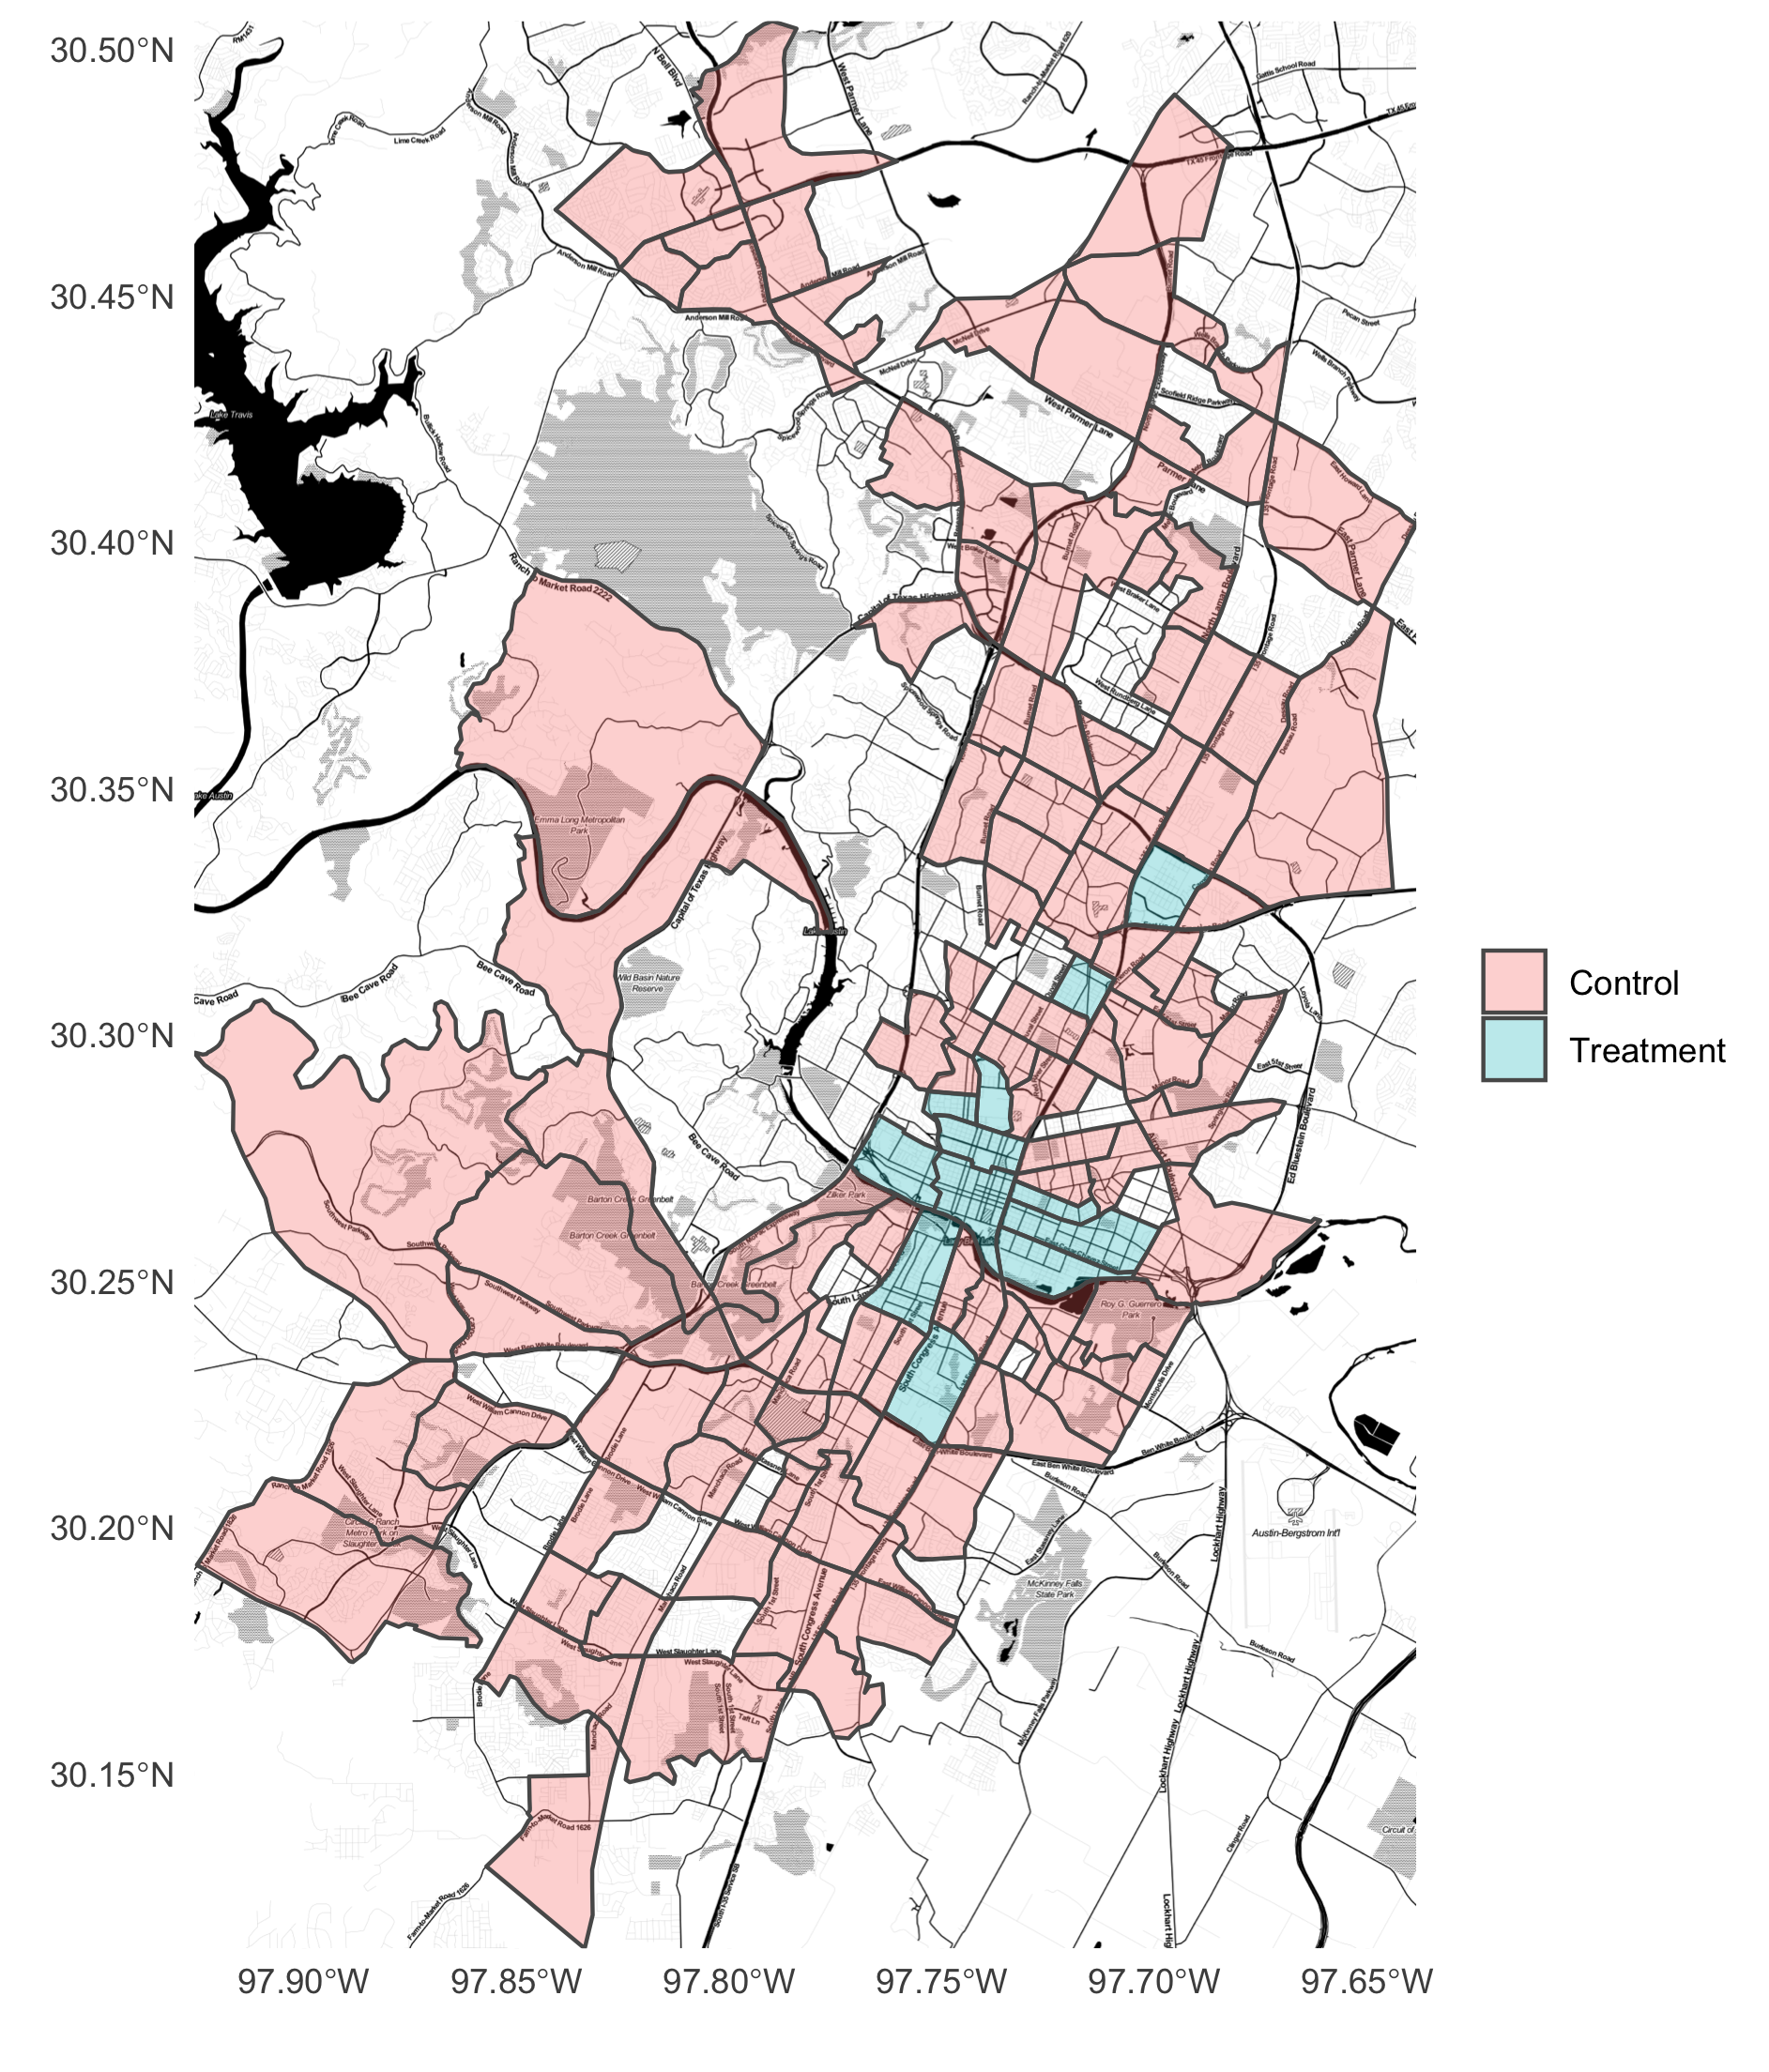
\includegraphics[width=\textwidth]{../../figures/treatment_by_tract.png}
    \end{center}
    \caption{Map of treated and control areas of Austin according to pre-treatment citation levels. Note the main treated areas are near Downtown Austin and the University of Texas.}
    \label{fig:treatment_by_tract}
\end{figure}


\begin{table}
    \begin{center}
        
\begin{tabular}{ccc}
    Cutoff Date     &   Estimate   &   Std Error \\ \toprule
    June 28, 2018   &   3.1285164        &   2.584715 \\
    June 20, 2019   &   3.5410402        &   2.8821456 \\ \bottomrule
\end{tabular}

    \end{center}
    \caption{Point estimates and bootstrap standard errors of OLS DID estimate}
    \label{tab:did_1}
\end{table}

\subsection{Identifying Assumptions}

In order to identify our model we must make both the typical strict exogeneity assumption of a fixed-effect model and the parallel trends assumption of a difference-in-difference model. Conditional on the tract-level fixed effect, we are assuming that absent the ordinance reform, high-homelessness census tracts would have experienced the same change in crime as the low-homelessness tracts. The strict exogeneity assumption implies that unobservables are uncorrelated across time, or that \(E(\varepsilon_{it}\varepsilon_{is}) = 0,\; \forall i,\; t\ne s\). In other words, we are assuming that there were no other unobservable changes, outside of the treatment effect, which shifted the number of crimes committed in the city. Inclusion of data from 2020 would cast doubt on my identifying assumptions, since the onset of COVID-19 appears to have had confounding implications on both encampment decisions of the homeless and the crime rate.

While I make no claim to be an expert in empirical crime studies, I think that both assumptions are more credible if conditioned on a larger set of covariates. Following a rational actor model of crime, we would expect opportunistic criminals to target higher-income and more densely populated areas. For Austin in particular, revelrous crowds of inebriated young adults are prime candidates for a pinch of thievery. In short, criminals and the unsheltered are drawn to the same parts of the city, albeit for different reasons. The introduction of a fixed effect is a crude way to control for this differential appeal. With more time I would draw tract-level characteristics from census data to make a more credible identification effort.

To illustrate identification of a difference-in-difference estimate in a fixed-effect framework, I present a classic breakdown in Table~\ref{tab:did_breakdown}, conducted on deviations from group means. This illustrates that inference is conducted in the model with respect to deviations from a time-invariant tract-level effect.

\begin{table}
    \begin{center}
        

\begin{tabular}{r|ccc}
    \toprule \multicolumn{4}{c}{}\\
    \multicolumn{4}{c}{Panel A: Using \(t^* = \) June 28, 2018} \\[1em]
             &           Treated                    &  Control                          &  Difference\\ \cmidrule(r){1-4}
    Before    & -1.3916667       &  -0.4531117   &  -0.9385549 \\
    After     & 3.2472222       &  1.0572607   &  2.1899615 \\
    Difference & 4.6388889 & 1.5103725 & 3.1285164 \\ \midrule\multicolumn{4}{c}{}\\

    \multicolumn{4}{c}{Panel B: Using \(t^* = \) June 20, 2019} \\[1em]
             &           Treated                    &  Control                          &  Difference\\ \cmidrule(r){1-4}
    Before    & -0.5243827       &  -0.1702787   &  -0.354104 \\
    After     & 4.7194444       &  1.5325083   &  3.1869362 \\
    Difference & 5.2438272 & 1.7027869 & 3.5410402 \\ \bottomrule
\end{tabular}

    \end{center}
    \caption{Difference-in-difference breakdown of demeaned monthly crime reports}
    \label{tab:did_breakdown}
\end{table}

\subsection{Event Study Robustness Check}

In order to provide a robustness check, I will use an event study design with a set of quarter-year time dummies spanning the 60 months in my sample. I estimate the model
\begin{equation*}
    y_{it} = \theta_0 + \theta_1 D_i + \sum_q 1(Q(t) = q)[\theta_{2q} + \delta_{q}D_i] + \alpha_i + \varepsilon_{it}
\end{equation*}
where \(Q(t)\) represents the quarter of month \(t\). I decide not to use month-year dummies because of the large parameter space this creates. I argue this does not significantly hinder interpretation: If there were some persistent treatment effect then we should see it even aggregating per quarter. I assign the treatment \(D_i\) based on the number of citations prior to June 28, 2018. Otherwise, results are not dependent on the choice of \(t^*\). Assigning the treatment areas using \(t^*=\)~June~20,~2019 did not significantly alter my findings.

\begin{figure}
    \begin{center}
        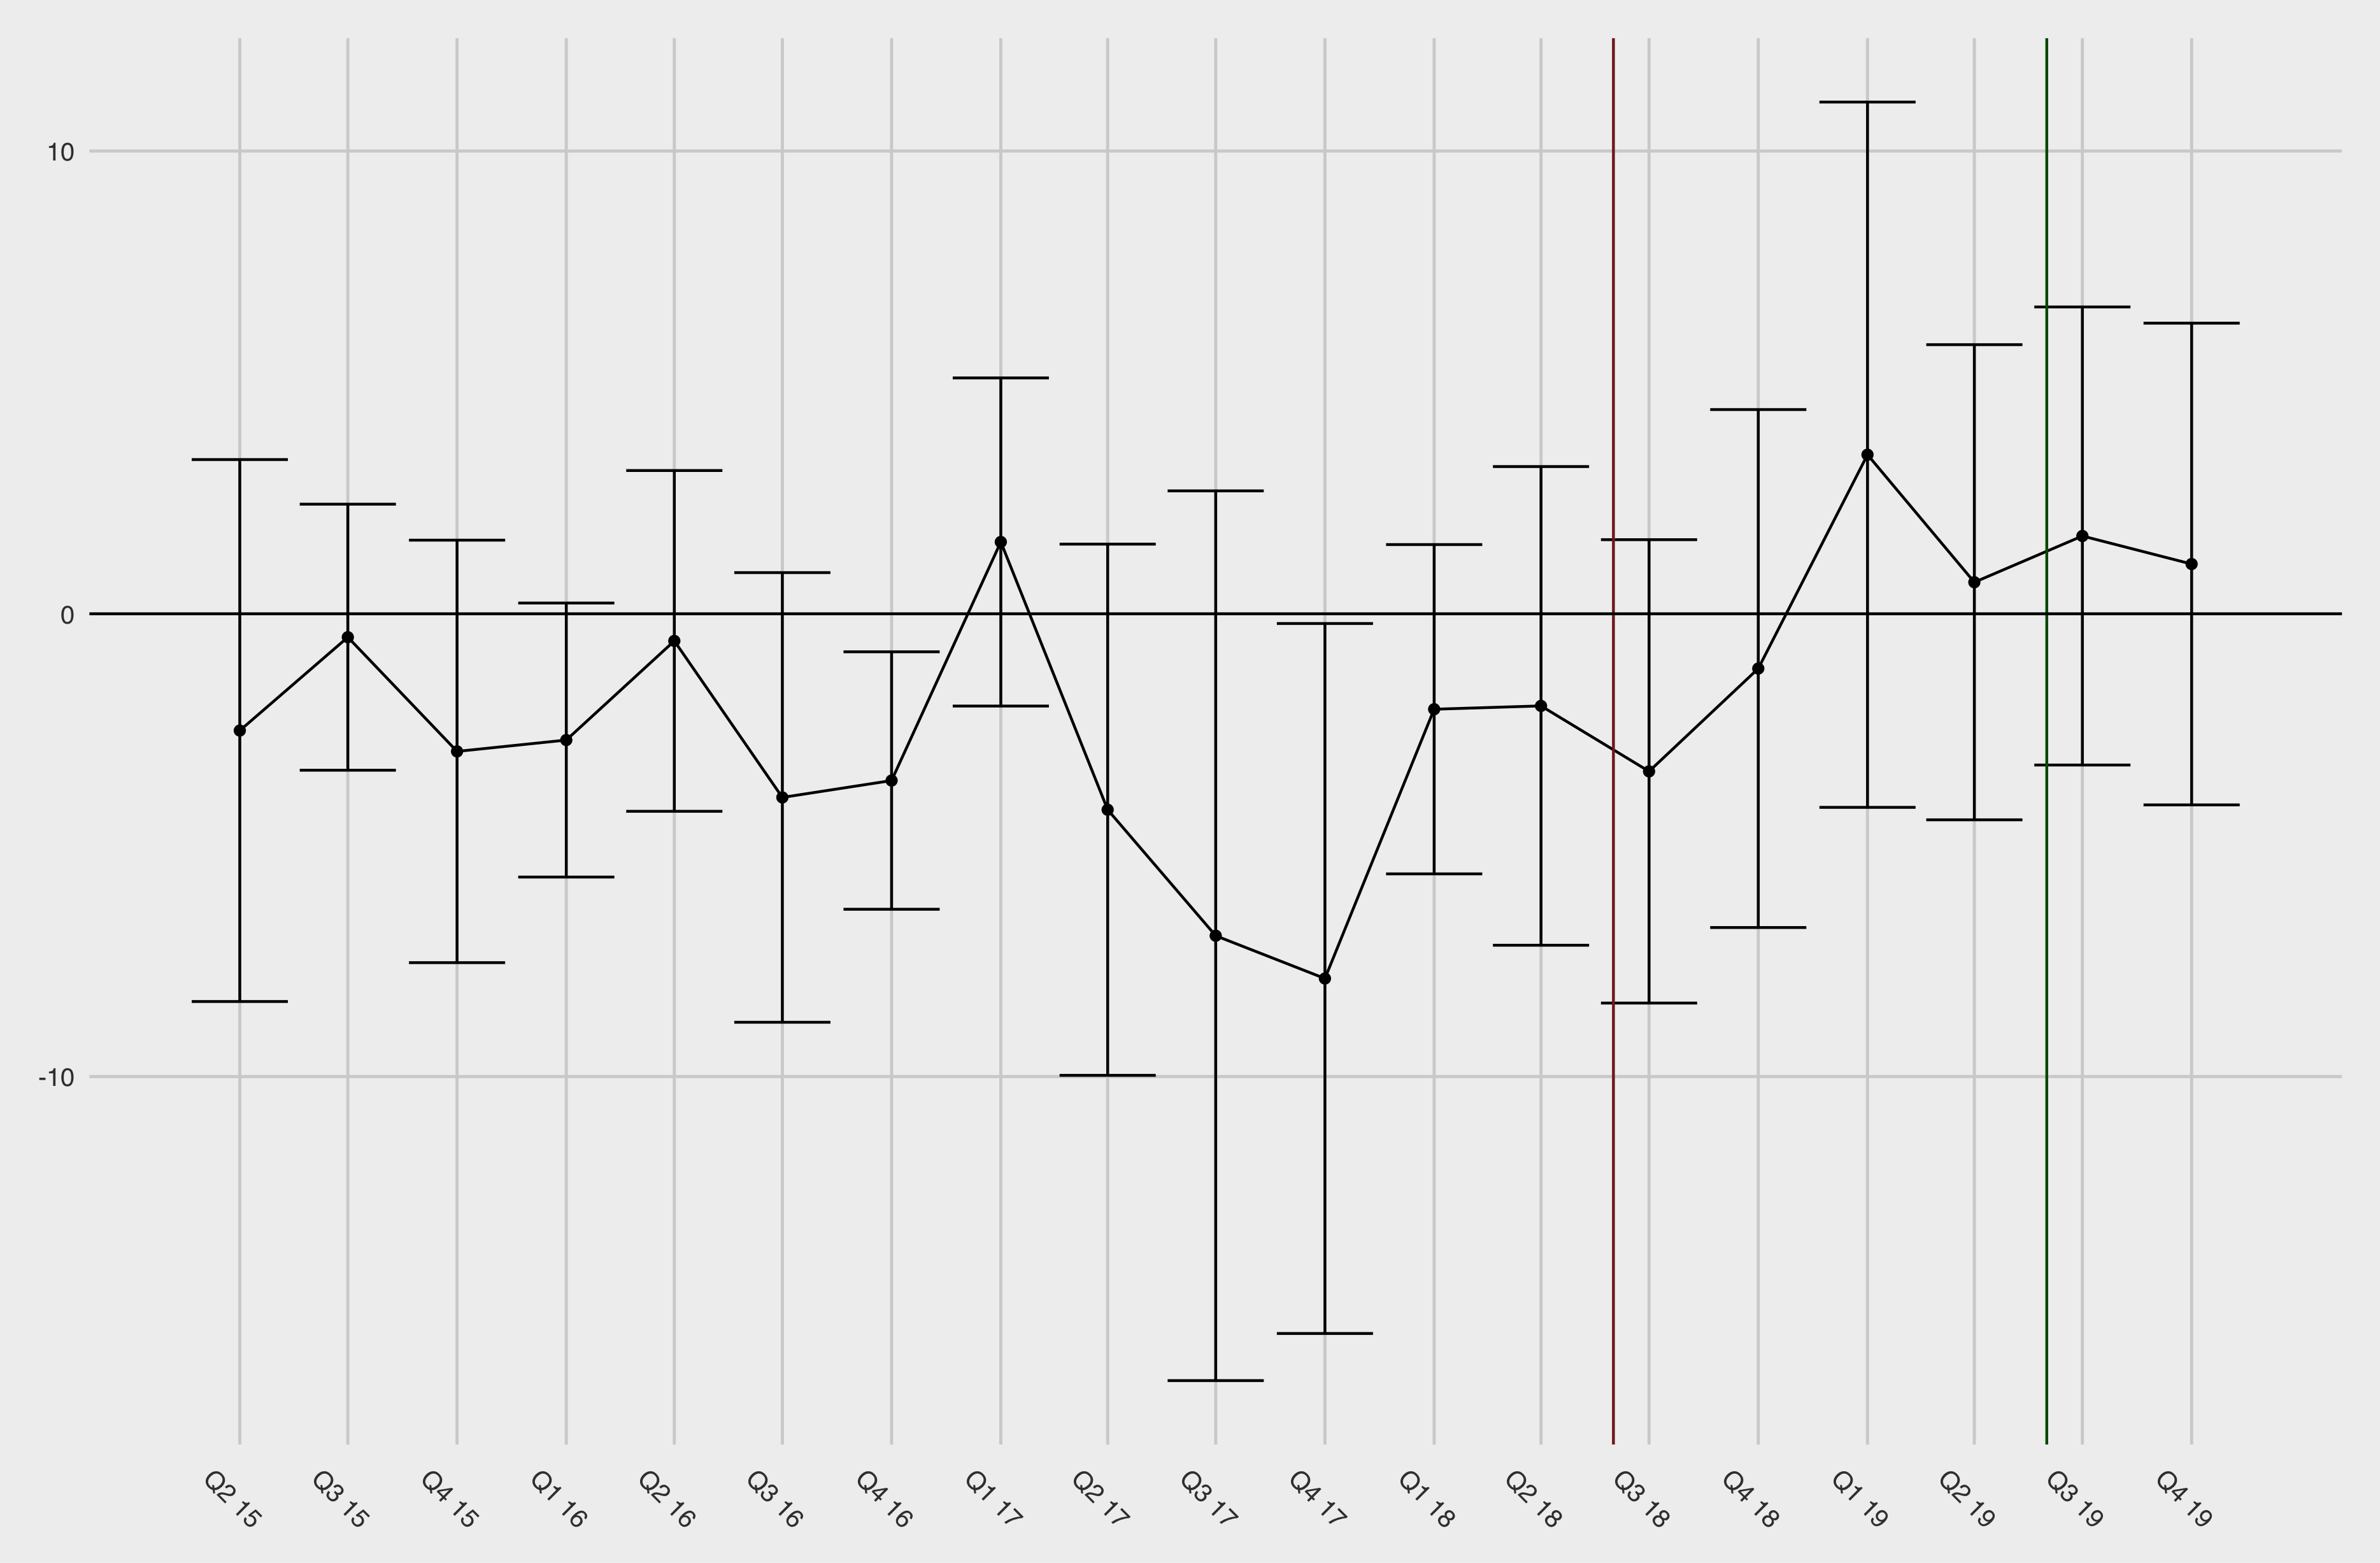
\includegraphics[width=\textwidth]{../../figures/event_study.png}
    \end{center}
    \caption{Treatment effect estimates using an event study design. Error bars denote a 95\% confidence interval using block bootstrapped standard errors. Red and green lines are June 28, 2018, and June 20, 2019, respectively.}
    \label{fig:event_study}
\end{figure}

Figure~\ref{fig:event_study} plots the 95\% confidence interval for each \(\delta_q\) estimate, using clustered bootstrap for standard error estimation. I drop the first quarter because of colinearity. All but two quarters in the pre-treatment period fail to differ significantly from zero. Point estimates do appear to move from negative to positive in the first quarter of 2019 and stay positive afterwards, but standard errors are large.